\documentclass[aspectratio=169, 10pt]{beamer}

% --- Core Packages ---
\usepackage[utf8]{inputenc}
\usepackage[T1]{fontenc}
\usepackage{lmodern}
\usepackage{amsmath, amssymb}
\usepackage{graphicx}
\usepackage{booktabs}
\usepackage{colortbl}
\usepackage{array}
\usepackage{tikz}
\usetikzlibrary{positioning, calc, shapes.geometric, backgrounds}
\usepackage[most]{tcolorbox}
\usepackage{fontawesome5}

% --- Color Palette (Dark Terminal Cybersecurity Theme) ---
\definecolor{bgdark}{HTML}{0B0F19}
\definecolor{bgcard}{HTML}{131B2E}
\definecolor{bgterminal}{HTML}{0A0D14}
\definecolor{cybercyan}{HTML}{38BDF8}
\definecolor{cybergreen}{HTML}{22C55E}
\definecolor{cyberamber}{HTML}{F59E0B}
\definecolor{cyberred}{HTML}{EF4444}
\definecolor{cyberpurple}{HTML}{A78BFA}
\definecolor{textlight}{HTML}{F3F4F6}
\definecolor{textmuted}{HTML}{9CA3AF}
\definecolor{borderdark}{HTML}{1E293B}

% --- Beamer Color & Font Customization ---
\setbeamercolor{background canvas}{bg=bgdark}
\setbeamercolor{normal text}{fg=textlight}
\setbeamercolor{frametitle}{fg=cybercyan, bg=bgdark}
\setbeamercolor{title}{fg=textlight}
\setbeamercolor{subtitle}{fg=cybercyan}
\setbeamercolor{author}{fg=textmuted}
\setbeamercolor{date}{fg=textmuted}
\setbeamercolor{structure}{fg=cybercyan}
\setbeamercolor{item}{fg=cybergreen}
\setbeamercolor{block title}{fg=cybercyan, bg=bgcard}
\setbeamercolor{block body}{fg=textlight, bg=bgcard}

% Disable Beamer Navigation Bar
\setbeamertemplate{navigation symbols}{}

% Custom Beamer List Bullet
\setbeamertemplate{itemize item}{\ttfamily\color{cybergreen}>}
\setbeamertemplate{itemize subitem}{\ttfamily\color{cybercyan}-}

% --- Custom Frame Title Header ---
\setbeamertemplate{frametitle}{
  \vspace*{2pt}%
  \begin{tcolorbox}[
    enhanced,
    colback=bgcard,
    colframe=borderdark,
    arc=3pt,
    boxrule=0.6pt,
    left=8pt, right=8pt, top=3pt, bottom=3pt
  ]
    \begin{minipage}{0.72\textwidth}
      {\ttfamily\color{cybercyan}\small \$ \insertframetitle}
    \end{minipage}\hfill
    \begin{minipage}{0.25\textwidth}
      \raggedleft
      {\ttfamily\color{textmuted}\tiny APEX-SEC // LABS}
    \end{minipage}
  \end{tcolorbox}
  \vspace*{-8pt}
}

% --- Custom Footline Footer ---
\setbeamertemplate{footline}{
  \begin{beamercolorbox}[wd=\paperwidth, ht=13pt, dp=3pt, leftskip=10pt, rightskip=10pt]{footline}
    {\ttfamily\color{textmuted}\tiny apex@sec-node-01:\textasciitilde\$ \hspace{4pt}|\hspace{4pt} Zero-Trust \& Threat Hunting 2026 \hfill Slide \insertframenumber{} / \inserttotalframenumber}
  \end{beamercolorbox}
}

% --- Custom tcolorbox Styles ---
\newtcolorbox{terminalbox}[2][]{
  enhanced,
  colback=bgterminal,
  colframe=borderdark,
  coltitle=textlight,
  fonttitle=\ttfamily\bfseries\small,
  title={#2},
  arc=3pt,
  boxrule=0.8pt,
  left=7pt, right=7pt, top=4pt, bottom=4pt,
  overlay={
    \fill[color=cyberred] ([xshift=10pt, yshift=-7pt]frame.north west) circle (2.2pt);
    \fill[color=cyberamber] ([xshift=17pt, yshift=-7pt]frame.north west) circle (2.2pt);
    \fill[color=cybergreen] ([xshift=24pt, yshift=-7pt]frame.north west) circle (2.2pt);
  },
  #1
}

\newtcolorbox{cybercard}[2][]{
  enhanced,
  colback=bgcard,
  colframe=cybercyan!40!bgcard,
  coltitle=cybercyan,
  fonttitle=\bfseries\small,
  title={#2},
  arc=3pt,
  boxrule=0.8pt,
  left=7pt, right=7pt, top=4pt, bottom=4pt,
  #1
}

\newtcolorbox{alertcard}[2][]{
  enhanced,
  colback=bgcard,
  colframe=cyberred!60!bgcard,
  coltitle=cyberred,
  fonttitle=\bfseries\small,
  title={#2},
  arc=3pt,
  boxrule=0.8pt,
  left=7pt, right=7pt, top=4pt, bottom=4pt,
  #1
}

\newtcolorbox{metricbox}[2][]{
  enhanced,
  colback=bgcard,
  colframe=cybercyan!50!bgcard,
  arc=3pt,
  boxrule=0.8pt,
  left=4pt, right=4pt, top=4pt, bottom=4pt,
  halign=center,
  #1
}

\begin{document}

% ==========================================
% SLIDE 1: TITLE SLIDE
% ==========================================
\begin{frame}[plain]
  \vfill
  \begin{terminalbox}{root@apex-sec-lab:\textasciitilde/strategy-2026\# ./init\_deck.sh}
    \vspace{4pt}
    \begin{center}
      {\ttfamily\color{cybercyan}\Large\bfseries ZERO-TRUST ARCHITECTURE \& THREAT HUNTING}\\[3pt]
      {\color{textmuted}\small Next-Generation Cloud Infrastructure Defense \& Continuous Attestation}\\[8pt]
      
      \begin{tcolorbox}[colback=bgcard, colframe=borderdark, arc=2pt, width=0.88\textwidth, halign=center, top=3pt, bottom=3pt]
        {\ttfamily\color{cybergreen}\small STATUS: ACTIVE \hspace{8pt}|\hspace{8pt} CLEARANCE: CONFIDENTIAL \hspace{8pt}|\hspace{8pt} VER: 4.2.0}
      \end{tcolorbox}
      \vspace{6pt}
      
      \begin{columns}
        \begin{column}{0.45\textwidth}
          \raggedright
          {\small\bfseries Presented By:}\\[1pt]
          {\color{cybercyan}\small Dr. Alex Mercer} {\color{textmuted}\tiny (Principal Architect, Apex Lab)}\\[1pt]
          {\color{cybercyan}\small Elena Rostova} {\color{textmuted}\tiny (Lead Threat Analyst, Vertex Security)}
        \end{column}
        \begin{column}{0.45\textwidth}
          \raggedleft
          {\small\bfseries Target Environment:}\\[1pt]
          {\color{textlight}\small Project Meridian Infrastructure}\\[1pt]
          {\color{textmuted}\tiny July 2026 // Global Cyber Operations}
        \end{column}
      \end{columns}
    \end{center}
    \vspace{2pt}
  \end{terminalbox}
  \vfill
\end{frame}

% ==========================================
% SLIDE 2: EXECUTIVE SUMMARY
% ==========================================
\begin{frame}{Executive Summary: The Threat Environment}
  \begin{columns}[T]
    \begin{column}{0.48\textwidth}
      \begin{cybercard}{\faLock\ \ Primary Objectives}
        \begin{itemize}
          \item Eliminate implicit trust boundaries across multi-cloud setups.
          \item Enforce micro-segmentation at compute boundaries.
          \item Implement automated pipelines with sub-minute containment.
          \item Continuous identity attestation using Ephemeral PKI tokens.
        \end{itemize}
      \end{cybercard}
    \end{column}
    \begin{column}{0.48\textwidth}
      \begin{alertcard}{\faExclamationTriangle\ \ 2026 Key Risk Vectors}
        \begin{itemize}
          \item API Credential Leakage in CI/CD pipelines (+42\% YoY).
          \item Non-Human Identity (NHI) key escalation in microservices.
          \item Supply chain compromise via unverified container registries.
          \item Lateral movement through over-privileged service accounts.
        \end{itemize}
      \end{alertcard}
    \end{column}
  \end{columns}

  \vspace{4pt}
  \begin{terminalbox}{syslog@vertex-node-04:\textasciitilde\$ tail -n 2 /var/log/audit.log}
    {\ttfamily\color{cyberamber}\small [ALERT] Unauthenticated API call from 192.0.2.145 to /v2/keys (Blocked by PDP)}\\[1pt]
    {\ttfamily\color{cybergreen}\small [INFO] Session token revoked for service-account:synapse-worker-09}
  \end{terminalbox}
\end{frame}

% ==========================================
% SLIDE 3: AGENDA
% ==========================================
\begin{frame}{Presentation Roadmap}
  \begin{terminalbox}{cat /etc/cyber-deck/agenda.conf}
    \vspace{1pt}
    \begin{enumerate}
      \item[\color{cybercyan}\ttfamily \lbrack 01\rbrack] {\bfseries Modern Threat Landscape \& Vector Analysis} \\
      {\color{textmuted}\small Cloud API risks, identity sprawl, and non-human credential abuse.} \vspace{3pt}
      
      \item[\color{cybercyan}\ttfamily \lbrack 02\rbrack] {\bfseries Zero-Trust Architecture Foundations} \\
      {\color{textmuted}\small Policy Decision Points (PDP), micro-segmentation, and ephemeral authentication.} \vspace{3pt}
      
      \item[\color{cybercyan}\ttfamily \lbrack 03\rbrack] {\bfseries Real-Time Telemetry \& Threat Hunting} \\
      {\color{textmuted}\small eBPF kernel tracing, log enrichment, and automated anomaly detection.} \vspace{3pt}
      
      \item[\color{cybercyan}\ttfamily \lbrack 04\rbrack] {\bfseries Automated Remediation \& Playbooks} \\
      {\color{textmuted}\small SOAR integration, microservice isolation, and automated token revocation.} \vspace{3pt}
      
      \item[\color{cybercyan}\ttfamily \lbrack 05\rbrack] {\bfseries Case Study: Project Meridian Deployment} \\
      {\color{textmuted}\small Production metrics, incident MTTR reduction, and enterprise security posture.}
    \end{enumerate}
  \end{terminalbox}
\end{frame}

% ==========================================
% SLIDE 4: SECTION 1 DIVIDER
% ==========================================
\begin{frame}[plain]
  \vfill
  \begin{tcolorbox}[
    enhanced,
    colback=bgcard,
    colframe=cybercyan,
    arc=4pt,
    boxrule=1.2pt,
    left=15pt, right=15pt, top=15pt, bottom=15pt
  ]
    {\ttfamily\color{cybercyan}\large SECTION 01} \\[4pt]
    {\Huge\bfseries\color{textlight} Modern Threat Landscape} \\[8pt]
    {\color{textmuted}\small Cloud-native attack surfaces, identity exploitation, and telemetry gaps.}
  \end{tcolorbox}
  \vfill
\end{frame}

% ==========================================
% SLIDE 5: ATTACK VECTORS & ANALYSIS
% ==========================================
\begin{frame}{Cloud-Native Attack Surface Expansion}
  \begin{columns}[T]
    \begin{column}{0.48\textwidth}
      \begin{terminalbox}{cat /var/data/vectors\_identity.json}
        {\ttfamily\color{cybercyan}\bfseries 1. Non-Human Identities (NHI)}
        \begin{itemize}
          \item Service accounts outnumber human users 15 to 1.
          \item Long-lived API keys unrotated for $>180$ days.
          \item Over-scoped IAM roles grant blanket admin rights.
        \end{itemize}
      \end{terminalbox}
    \end{column}
    \begin{column}{0.48\textwidth}
      \begin{terminalbox}{cat /var/data/vectors\_infra.json}
        {\ttfamily\color{cyberamber}\bfseries 2. Container \& Kubernetes Risks}
        \begin{itemize}
          \item Misconfigured Pod Security Standards (PSS).
          \item Exposed Kubelet APIs and open endpoints.
          \item Vulnerabilities in third-party base images.
        \end{itemize}
      \end{terminalbox}
    \end{column}
  \end{columns}

  \vspace{4pt}
  \begin{tcolorbox}[colback=bgcard, colframe=borderdark, arc=3pt, left=7pt, right=7pt, top=3pt, bottom=3pt]
    {\small\color{cybercyan}\faKey\ \ \textbf{Key Takeaway:}} {\small Traditional perimeter firewalls cannot inspect microservice east-west traffic effectively.}
  \end{tcolorbox}
\end{frame}

% ==========================================
% SLIDE 6: THREAT ACTOR MATRIX (TABLE)
% ==========================================
\begin{frame}{TTP Analysis \& Threat Actor Profile}
  \vspace{-4pt}
  {\small\color{textmuted} Analysis of observed tactics, techniques, and procedures across enterprise environments:}
  \vspace{4pt}
  
  \begin{center}
    \small
    \rowcolors{2}{bgcard}{bgterminal}
    \begin{tabular}{lp{3.5cm}p{3.8cm}cc}
      \toprule
      \color{cybercyan}\textbf{Tactic ID} & \color{cybercyan}\textbf{Attack Vector} & \color{cybercyan}\textbf{Primary Target} & \color{cybercyan}\textbf{Risk Level} & \color{cybercyan}\textbf{Mitigation Status} \\
      \midrule
      T1078 & Credential Access & CI/CD Pipeline Tokens & \color{cyberred}\textbf{CRITICAL} & \color{cybergreen}Enforced Ephemeral \\{}
      T1190 & Exploit Public App & Ingress Gateway Endpoints & \color{cyberred}\textbf{HIGH} & \color{cybergreen}WAF + PDP Filter \\{}
      T1068 & Privilege Escalation & Container Host Kernel & \color{cyberamber}\textbf{MEDIUM} & \color{cybergreen}eBPF Seccomp Profile \\{}
      T1020 & Data Exfiltration & Database Replica Endpoints & \color{cyberred}\textbf{HIGH} & \color{cybergreen}mTLS + DLP Sensor \\{}
      T1496 & Resource Hijacking & Unused Compute Nodes & \color{cyberamber}\textbf{LOW} & \color{cybergreen}Auto-Scaling Limit \\
      \bottomrule
    \end{tabular}
  \end{center}

  \vspace{4pt}
  \begin{cybercard}{\faLock\ \ Defense Posture Summary}
    {\small 100\% of high-risk vectors are mapped directly to continuous policy decision enforcement points.}
  \end{cybercard}
\end{frame}

% ==========================================
% SLIDE 7: SECTION 2 DIVIDER
% ==========================================
\begin{frame}[plain]
  \vfill
  \begin{tcolorbox}[
    enhanced,
    colback=bgcard,
    colframe=cybergreen,
    arc=4pt,
    boxrule=1.2pt,
    left=15pt, right=15pt, top=15pt, bottom=15pt
  ]
    {\ttfamily\color{cybergreen}\large SECTION 02} \\[4pt]
    {\Huge\bfseries\color{textlight} Zero-Trust Architecture Foundations} \\[8pt]
    {\color{textmuted}\small Never trust, always verify: Identity attestation, PDP/PEP enforcement, and micro-segmentation.}
  \end{tcolorbox}
  \vfill
\end{frame}

% ==========================================
% SLIDE 8: THREE PILLARS OF ZERO TRUST
% ==========================================
\begin{frame}{The Core Pillars of Zero-Trust}
  \begin{columns}[T]
    \begin{column}{0.31\textwidth}
      \begin{cybercard}{\faUserCheck\ \ 1. Identity Attestation}
        \begin{itemize}
          \item Dynamic mTLS certificate gen.
          \item Short-lived SPIFFE IDs.
          \item Hardware TPM key storage.
        \end{itemize}
      \end{cybercard}
    \end{column}

    \begin{column}{0.31\textwidth}
      \begin{cybercard}{\faNetworkWired\ \ 2. Micro-segmentation}
        \begin{itemize}
          \item L4 and L7 network policies.
          \item Default-deny rule engine.
          \item Service-mesh proxies.
        \end{itemize}
      \end{cybercard}
    \end{column}

    \begin{column}{0.31\textwidth}
      \begin{cybercard}{\faSearch\ \ 3. Continuous Telemetry}
        \begin{itemize}
          \item Kernel-level eBPF tracing.
          \item Real-time behavior profile.
          \item Automated risk engine.
        \end{itemize}
      \end{cybercard}
    \end{column}
  \end{columns}

  \vspace{6pt}
  \begin{terminalbox}{zt-policy-check --service nexus-api}
    {\ttfamily\color{cybergreen}\small [PASSED] Identity token verified (SPIFFE: spiffe://apex.internal/sa/nexus-api)}\\[1pt]
    {\ttfamily\color{cybergreen}\small [PASSED] mTLS Handshake completed with Cipher: TLS\_AES\_256\_GCM\_SHA384}
  \end{terminalbox}
\end{frame}

% ==========================================
% SLIDE 9: TIKZ ARCHITECTURE DIAGRAM
% ==========================================
\begin{frame}{Zero-Trust Control \& Data Plane Architecture}
  \begin{center}
    \begin{tikzpicture}[
      scale=0.82, every node/.style={transform shape},
      node distance=1.4cm and 1.8cm,
      box/.style={draw=borderdark, fill=bgcard, rounded corners=3pt, thick, align=center, text=textlight, minimum width=2.3cm, minimum height=1.1cm, font=\sffamily\small},
      cyberbox/.style={draw=cybercyan, fill=bgcard, rounded corners=3pt, thick, align=center, text=textlight, minimum width=2.4cm, minimum height=1.1cm, font=\sffamily\small},
      pdpbox/.style={draw=cybergreen, fill=bgterminal, rounded corners=3pt, ultra thick, align=center, text=cybergreen, minimum width=2.6cm, minimum height=1.2cm, font=\ttfamily\bfseries\small},
      arrow/.style={->, >=stealth, thick, color=cybercyan},
      alertarrow/.style={->, >=stealth, dashed, thick, color=cyberamber}
    ]

      % Background Group Box drawn manually using coordinates
      \draw [draw=borderdark, dashed, fill=bgdark!60!bgcard, rounded corners=5pt] (-0.3, -1.0) rectangle (11.8, 2.4);
      \node [font=\tiny\ttfamily\color{textmuted}, anchor=south east] at (11.7, -0.9) {Protected Zero-Trust Boundary};

      % Nodes
      \node (client) [box] {\faDesktop\\Client App};
      \node (ingress) [cyberbox, right=of client] {\faGlobe\\API Gateway\\(PEP)};
      \node (pdp) [pdpbox, above=0.9cm of ingress] {\faLock\ Policy Engine\\(PDP / OPA)};
      \node (serviceA) [box, right=of ingress] {\faServer\\Auth Service\\(Nexa Node)};
      \node (serviceB) [box, right=of serviceA] {\faDatabase\\Vault Service\\(Meridian Data)};

      % Connections
      \draw [arrow] (client) -- node[above, font=\tiny\ttfamily\color{textmuted}]{HTTPS / JWT} (ingress);
      \draw [arrow] (ingress) -- node[left, font=\tiny\ttfamily\color{cybercyan}]{Check Policy} (pdp);
      \draw [arrow] (ingress) -- node[above, font=\tiny\ttfamily\color{cybergreen}]{mTLS 1.3} (serviceA);
      \draw [arrow] (serviceA) -- node[above, font=\tiny\ttfamily\color{cybergreen}]{SPIFFE Token} (serviceB);
      
      \draw [alertarrow] (pdp) -| node[above, font=\tiny\ttfamily\color{cyberamber}, pos=0.25]{Telemetry Stream} (serviceB);
    \end{tikzpicture}
  \end{center}
  \vspace{-6pt}
  \begin{center}
    {\tiny\color{textmuted}\ttfamily PEP = Policy Enforcement Point | PDP = Policy Decision Point | OPA = Open Policy Agent | mTLS = Mutual TLS}
  \end{center}
\end{frame}

% ==========================================
% SLIDE 10: SECTION 3 DIVIDER
% ==========================================
\begin{frame}[plain]
  \vfill
  \begin{tcolorbox}[
    enhanced,
    colback=bgcard,
    colframe=cyberamber,
    arc=4pt,
    boxrule=1.2pt,
    left=15pt, right=15pt, top=15pt, bottom=15pt
  ]
    {\ttfamily\color{cyberamber}\large SECTION 03} \\[4pt]
    {\Huge\bfseries\color{textlight} Real-Time Telemetry \& Detection} \\[8pt]
    {\color{textmuted}\small eBPF event stream capture, rule evaluation, and log anomaly identification.}
  \end{tcolorbox}
  \vfill
\end{frame}

% ==========================================
% SLIDE 11: CODE & LOG FORENSICS
% ==========================================
\begin{frame}{Telemetry Analysis \& Detection Logic}
  \begin{columns}[T]
    \begin{column}{0.48\textwidth}
      \begin{terminalbox}{auditd\_event.json}
        {\ttfamily\tiny\color{textlight}
\{ \\
\ \ "timestamp": "2026-07-24T09:12:04Z", \\
\ \ "event\_type": "EXECVE", \\
\ \ "process": "/usr/bin/curl", \\
\ \ "parent": "synapse-worker-app", \\
\ \ "user": "www-data", \\
\ \ "cmdline": "curl -s http://169.254.169.254/", \\
\ \ "container\_id": "c9a8f42d11", \\
\ \ "threat\_score": 0.94 \\
\}
        }
      \end{terminalbox}
    \end{column}

    \begin{column}{0.48\textwidth}
      \begin{terminalbox}{detection\_rule.py}
        {\ttfamily\tiny\color{cybercyan}
def evaluate\_event(event): \\
\ \ \# Check for IMDS SSRF Attempt \\
\ \ if "169.254.169.254" in event.cmdline: \\
\ \ \ \ if event.user != "root\_admin": \\
\ \ \ \ \ \ emit\_alert( \\
\ \ \ \ \ \ \ \ severity="CRITICAL", \\
\ \ \ \ \ \ \ \ action="KILL\_CONTAINER", \\
\ \ \ \ \ \ \ \ target=event.container\_id \\
\ \ \ \ \ \ ) \\
\ \ \ \ \ \ return True \\
\ \ return False
        }
      \end{terminalbox}
    \end{column}
  \end{columns}

  \vspace{3pt}
  \begin{alertcard}{\faBug\ \ Anomaly Detected: Metadata SSRF Probing}
    {\small Automated rule matched execution pattern. Container \texttt{c9a8f42d11} isolated in 120ms.}
  \end{alertcard}
\end{frame}

% ==========================================
% SLIDE 12: SECURITY OPERATIONS BENCHMARKS
% ==========================================
\begin{frame}{Security Operations Benchmarks (2026 Targets)}
  \begin{columns}[T]
    \begin{column}{0.23\textwidth}
      \begin{metricbox}{}
        {\ttfamily\color{textmuted}\tiny MEAN TIME TO DETECT}\\[2pt]
        {\Huge\bfseries\color{cybercyan} 14s}\\[4pt]
        {\tiny\color{cybergreen}\faCheck\ -82\% vs 2025}
      \end{metricbox}
    \end{column}
    
    \begin{column}{0.23\textwidth}
      \begin{metricbox}{}
        {\ttfamily\color{textmuted}\tiny MEAN TIME TO RESPOND}\\[2pt]
        {\Huge\bfseries\color{cybergreen} 45s}\\[4pt]
        {\tiny\color{cybergreen}\faCheck\ Fully Automated}
      \end{metricbox}
    \end{column}

    \begin{column}{0.23\textwidth}
      \begin{metricbox}{}
        {\ttfamily\color{textmuted}\tiny FALSE POSITIVE RATE}\\[2pt]
        {\Huge\bfseries\color{cyberamber} 0.4\%}\\[4pt]
        {\tiny\color{cybergreen}\faCheck\ Tuned ML Rules}
      \end{metricbox}
    \end{column}

    \begin{column}{0.23\textwidth}
      \begin{metricbox}{}
        {\ttfamily\color{textmuted}\tiny TELEMETRY RATE}\\[2pt]
        {\Huge\bfseries\color{cyberpurple} 2.4M}\\[4pt]
        {\tiny\color{textmuted} events / second}
      \end{metricbox}
    \end{column}
  \end{columns}

  \vspace{8pt}
  \begin{terminalbox}{telemetry-status --cluster meridian-prod}
    {\ttfamily\color{cybergreen}\small [OK] eBPF Sensors active on 1,420 nodes | Zero loss buffer | Latency: 4.2ms}
  \end{terminalbox}
\end{frame}

% ==========================================
% SLIDE 13: SECTION 4 DIVIDER
% ==========================================
\begin{frame}[plain]
  \vfill
  \begin{tcolorbox}[
    enhanced,
    colback=bgcard,
    colframe=cyberpurple,
    arc=4pt,
    boxrule=1.2pt,
    left=15pt, right=15pt, top=15pt, bottom=15pt
  ]
    {\ttfamily\color{cyberpurple}\large SECTION 04} \\[4pt]
    {\Huge\bfseries\color{textlight} Automated Response Playbooks} \\[8pt]
    {\color{textmuted}\small Closed-loop mitigation: Isolation, key rotation, and patch deployment.}
  \end{tcolorbox}
  \vfill
\end{frame}

% ==========================================
% SLIDE 14: AUTOMATED RESPONSE PIPELINE
% ==========================================
\begin{frame}{Automated Incident Response Workflow}
  \begin{center}
    \begin{tikzpicture}[
      scale=0.88, every node/.style={transform shape},
      node distance=1.2cm,
      stepbox/.style={draw=borderdark, fill=bgcard, rounded corners=4pt, thick, align=center, text=textlight, minimum width=2.4cm, minimum height=1.3cm, font=\sffamily\small},
      arrow/.style={->, >=stealth, ultra thick, color=cybercyan}
    ]

      \node (step1) [stepbox, draw=cyberamber] {\ttfamily\color{cyberamber}STEP 01\\[2pt]\small\faExclamationTriangle\ Anomaly Detected};
      \node (step2) [stepbox, right=of step1, draw=cybercyan] {\ttfamily\color{cybercyan}STEP 02\\[2pt]\small\faSlidersH\ Risk Scoring};
      \node (step3) [stepbox, right=of step2, draw=cyberpurple] {\ttfamily\color{cyberpurple}STEP 03\\[2pt]\small\faLock\ Token Revocation};
      \node (step4) [stepbox, right=of step3, draw=cybergreen] {\ttfamily\color{cybergreen}STEP 04\\[2pt]\small\faMicrochip\ Pod Isolation};

      \draw [arrow] (step1) -- (step2);
      \draw [arrow] (step2) -- (step3);
      \draw [arrow] (step3) -- (step4);
    \end{tikzpicture}
  \end{center}

  \vspace{4pt}
  \begin{terminalbox}{soar-engine --playbook auto\_contain\_v4.yaml}
    \begin{itemize}
      \item[{\ttfamily\color{cybergreen}1.}] {\small\textbf{Revoke OAuth Token:} Invalidation across Redis cache nodes.}
      \item[{\ttfamily\color{cybergreen}2.}] {\small\textbf{Cilium Policy:} Apply drop-all egress rule to target.}
      \item[{\ttfamily\color{cybergreen}3.}] {\small\textbf{Memory Dump:} Capture volatile RAM state to S3 storage bucket.}
      \item[{\ttfamily\color{cybergreen}4.}] {\small\textbf{Ticket Gen:} Auto-create P1 incident in Vertex Ops Center.}
    \end{itemize}
  \end{terminalbox}
\end{frame}

% ==========================================
% SLIDE 15: CASE STUDY - PROJECT MERIDIAN
% ==========================================
\begin{frame}{Case Study: Project Meridian Production Rollout}
  \begin{columns}[T]
    \begin{column}{0.48\textwidth}
      \begin{alertcard}{Legacy Infrastructure (Pre-2026)}
        \begin{itemize}
          \item Perimeter firewall with flat internal network.
          \item Static 90-day API keys for microservices.
          \item Manual SOC triage (avg MTTR: 4.2 hours).
          \item Audits performed once per quarter.
        \end{itemize}
      \end{alertcard}
    \end{column}

    \begin{column}{0.48\textwidth}
      \begin{cybercard}{Zero-Trust Mesh (Post-2026)}
        \begin{itemize}
          \item Granular L7 network micro-segmentation.
          \item Ephemeral SPIFFE tokens (15-min TTL).
          \item Automated SOAR playbook (avg MTTR: 45s).
          \item Continuous real-time compliance attestation.
        \end{itemize}
      \end{cybercard}
    \end{column}
  \end{columns}

  \vspace{4pt}
  \begin{tcolorbox}[colback=bgcard, colframe=cybergreen, arc=3pt, left=7pt, right=7pt, top=3pt, bottom=3pt]
    {\small\color{cybergreen}\faCheck\ \textbf{Outcome:}} {\small Zero unauthorized lateral movement incidents recorded during Q2 2026 Red Team audit.}
  \end{tcolorbox}
\end{frame}

% ==========================================
% SLIDE 16: STRATEGIC ROADMAP
% ==========================================
\begin{frame}{Strategic Security Roadmap \& Checklist}
  \begin{terminalbox}{cat /opt/apex/roadmap\_checklist.md}
    \begin{itemize}
      \item[\color{cybergreen}\ttfamily \lbrack X\rbrack] {\bfseries Phase 1: Identity \& Ephemeral Credentials} \\
      {\color{textmuted}\small Complete migration from static keys to SPIFFE/SPIRE PKI tokens.} \vspace{2pt}
      
      \item[\color{cybergreen}\ttfamily \lbrack X\rbrack] {\bfseries Phase 2: eBPF Telemetry Sensor Deployment} \\
      {\color{textmuted}\small Deploy kernel event filters across all Kubernetes worker nodes.} \vspace{2pt}
      
      \item[\color{cyberamber}\ttfamily \lbrack >\rbrack] {\bfseries Phase 3: Automated East-West Policy Tuning} \\
      {\color{textmuted}\small Transition from audit mode to enforcing default-deny in production.} \vspace{2pt}
      
      \item[\color{cybercyan}\ttfamily \lbrack\ \rbrack] {\bfseries Phase 4: AI Threat Simulation \& Red Teaming} \\
      {\color{textmuted}\small Implement continuous adversarial validation pipelines.}
    \end{itemize}
  \end{terminalbox}
\end{frame}

% ==========================================
% SLIDE 17: CLOSING & Q&A
% ==========================================
\begin{frame}[plain]
  \vfill
  \begin{terminalbox}{root@apex-sec-lab:\textasciitilde\# ./shutdown\_presentation.sh --success}
    \vspace{8pt}
    \begin{center}
      {\ttfamily\Huge\bfseries\color{cybercyan} THANK YOU} \\[6pt]
      {\color{textlight}\Large Questions \& Discussion} \\[12pt]
      
      \begin{tcolorbox}[colback=bgcard, colframe=borderdark, arc=3pt, width=0.85\textwidth, halign=center, top=4pt, bottom=4pt]
        {\ttfamily\color{cybergreen}\small CONTACT \& LAB RESOURCES} \\[2pt]
        {\small\color{textlight} Apex Cyber Security Research Lab // Vertex Security Alliance} \\[1pt]
        {\ttfamily\color{cybercyan}\small Email: contact@apex-sec.internal \hspace{8pt}|\hspace{8pt} Docs: https://meridian.apex.internal}
      \end{tcolorbox}
      \vspace{8pt}
      
      {\ttfamily\color{textmuted}\small Session Terminated Successfully. Press [ESC] to Exit.}
    \end{center}
    \vspace{4pt}
  \end{terminalbox}
  \vfill
\end{frame}

\end{document}
